\chapter{Frequency disparity-coherent watermarking}
\markright{Frequency disparity-coherent watermarking}
\label{dft}
\phantomsection

Is now proposed a variant of the described watermarking process, which works in the frequency domain.

\section{ALGORITMO DEL PROF}

The strategy is based on the technique presented by Piva et al in "Improving DFT Watermarking robustness through optimum detection and synchronisation" [], where a watermarking algorithm for digital images operating in the frequency domain is presented: the method embeds a pseudo-random sequence of real numbers in a selected set of DFT coefficients of the image. Moreover, a synchronisation pattern is embedded into the watermarked image, to cope with geometrical attacks, like resizing and rotation. After embedding, the watermark is adapted to the image by exploiting the masking characteristics of the Human Visual System, thus ensuring the watermark invisibility.\newline
\begin{figure}[h!]
\centering
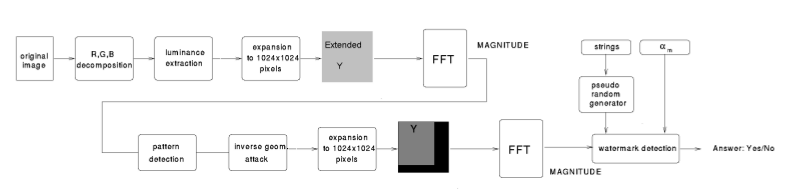
\includegraphics[width=0.9\textwidth]{./img/blocchi.png}
\caption{\small{watermarking algorithm}}
\label{fig:blocchi}
\end{figure}

For the stereo watermarking task this process has been simplified and cut to the basic frequency watermaking.

\subsection{Watermark embedding}

In [] the watermark is embedded in a subset of DFT coefficients of the luminance $Y$.\newline Since a traslation of the scene will only change the phase values of the DFT, leaving unaltered the magnitude values, the watermak only concernes the latter, to achieve robustness against image traslation.\newline
To garantee a blind detection system the number and position of the coefficient are fixed a priori: based on the size of the image to watermark, the coefficient are choosen in the medium frequencies of the spectrum to achieve a compromise between robustness and invisibillity.\newline 
The watermark embedding rule is the following:
$$y_{i}^{'} = y_{i}+\alpha m_{i}y_{i} $$
where $y_{i}^{'}$ represents the watermarked DFT magnitude coefficient, $y_{i}$ the corresponding original, $m_{i}$ is a sample of the watermark sequence, and $\alpha$ is the watermark energy.\newline
The inverted DFT is then applied to obtain the watermarked luminance $Y^{'}$.

\subsection{Watermark detection}

To determine if a given image luminance $Y$ either embedds or not the reference watermark in [] is used a threshold-based detection.\newline
From the received image is extracted the luminance of which is computed the DFT transform; from the obtained magnitude matrix the right coefficents can be selected since their position is fixed a priori as said above.\newline
Knowing the seed (in the shape of two strings, one numeric one alphanumeric) the watermark can be reproduced.\newline

To verify if the selected coefficients have been altered with the watermark its used a statistical decision theory: two hypotheses are defined, the image contains the reference watermark (hypotheses H1) or the image does not contain this mark (hypotheses H0). Relying on Bayes theory of hypothesis testing, the optimum criterion to test H1 versus H0 is minimum Bayes risk; the test function results to be the likelihood ratio function L that has to be compared to a threshold:\newline
\begin{itemize}
\item if $L > \lambda$ ,  the watermark $m^{*}$ is present;
\item if $L < \lambda$ , the watermark  $m^{*}$ is absent.
\end{itemize}

To choose a proper threshold, its been chosen to fix a constraint on the maximum false positive probability and the optimum decoder is designed refferring to the to the Neyman-Pearson criterion: \newline

$$ L(y)=\sum_{i=0}^{N-1} [-\beta ln(1+\alpha_{m}m_{i}^{*})]+\sum_{i=0}^{N-1}[-(\frac{y_{i}}{\alpha_{i}(1+\alpha_{m}m_{i}^{*})}))^{\beta_{i}}+(\frac{y_{i}}{\alpha_{i}})^{\beta_{i}}] $$
and
$$\lambda=3.3\sqrt{2\sum_{i=0}^{N-1}[\frac{[(1+\alpha_{m}m_{i}^{*})^{\beta_{i}}]}{(1+\alpha_{m}m_{i}^{*})^{\beta_{i}}}]} + \sum_{i=0}^{N-1}\{\frac{[(1+\alpha_{m}m_{i}^{*})^{\beta_{i}}-1]}{(1+\alpha_{m}m_{i}^{*})^{\beta_{i}}}\} - \sum_{i=0}^{N-1}[\beta_{i}ln(1+\alpha_{m}m_{i}^{*})]$$

In ()  $m^{*} = \{ m^{*}_{i} \} i= 0,1,...N-1$ is the watermark, $\alpha_{m}$ the mean watermark energy, $\alpha_{i}$ and $\beta_{i}$ are statistic parameters describing the probability density function shape of the magnitude of the watermarked DFT coefficients $y_{i}$.\newline 
The values of this parameters are choosen by means of Maximum Likelihood criterion, based on the the fact that the coefficients belonging to small
sub-regions of the spectrum are characterised by the same statistic parameters and follows a Weibull distribution:
$$ f(y_{i}) = \frac{\beta}{\alpha}(\frac{y_{i}}{\alpha})^{\beta-1}\exp\{-(\frac{y_{i}}{\alpha})^{\beta}\}$$
In summary, the detection process can be decomposed in the following steps:
\begin{itemize}
\item generation of the watermark $m^{*}$;
\item estimation of the parameters $\alpha,\beta$ into the regions composing the watermarked area of the spectrum;
\item computation of $L(y)$ and $\lambda$ ;
\item comparison between $L(y)$ and $\lambda$ ;
\item decision.
\end{itemize}

The decoder can detect the watermark presence also in highly degraded images. In particular, the system is robust to sequences of different attacks, such as rotation, resizing, and JPEG compression, or such as cropping, resizing and median filtering.

\section{Stereo watermarking algorithm}

For the stero-marking process its been taken under consideration a 512x512 subset of pixel of the image, in particular we focused in marking the part of the scene which is common to both the left and right view.

\begin{figure}[h!]
\centering
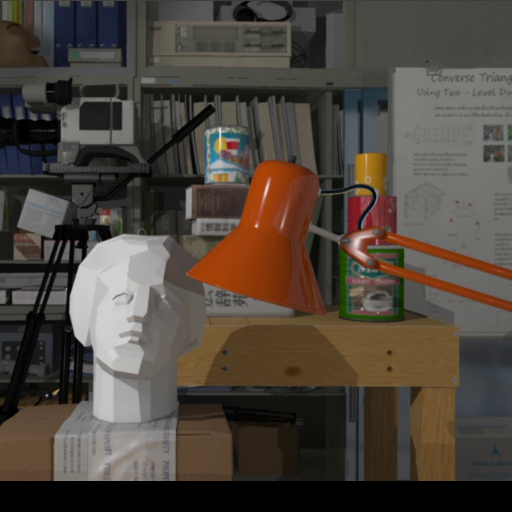
\includegraphics[width=0.5\textwidth]{./img/squared.png}
\caption{\small{cropped image to watermark}}
\label{fig:cropped}
\end{figure}

The left view is then processed with the algorithm discribed above.\newline 

To watermark the right view the pattern is created ad-hoc: a signal of the watermak is generated using the phase of the left image and the phase of the reference watermark and  the coefficients of the right view.\newline  
This way the right view will be marked with its coefficient, but with the correct phase, and the corresponding pixel in the left and right view will present the same alteration, not to cause visual distorsions.

$$ l_{w} = l + \frac{1}{MN}\sum\sum(\alpha|L(u,v)||w|\exp\{j(\phi_{l}+\phi_{w})\})\exp\{+j2\pi(\frac{ux}{M}\frac{vy}{N})\} $$
$$ r_{w} = r + \frac{1}{MN}\sum\sum(\alpha|R(u,v)||w|\exp\{j(\phi_{l}+\phi_{w})\})^{*}\exp\{+j2\pi(\frac{ux}{M}\frac{vy}{N})\} $$


The watermark is then brought back in the spatial domain with the inverse Fourier trasform, the image is warped according to the left-to-right disparity and added spatially to the right view.
\begin{figure}[h!]
\centering
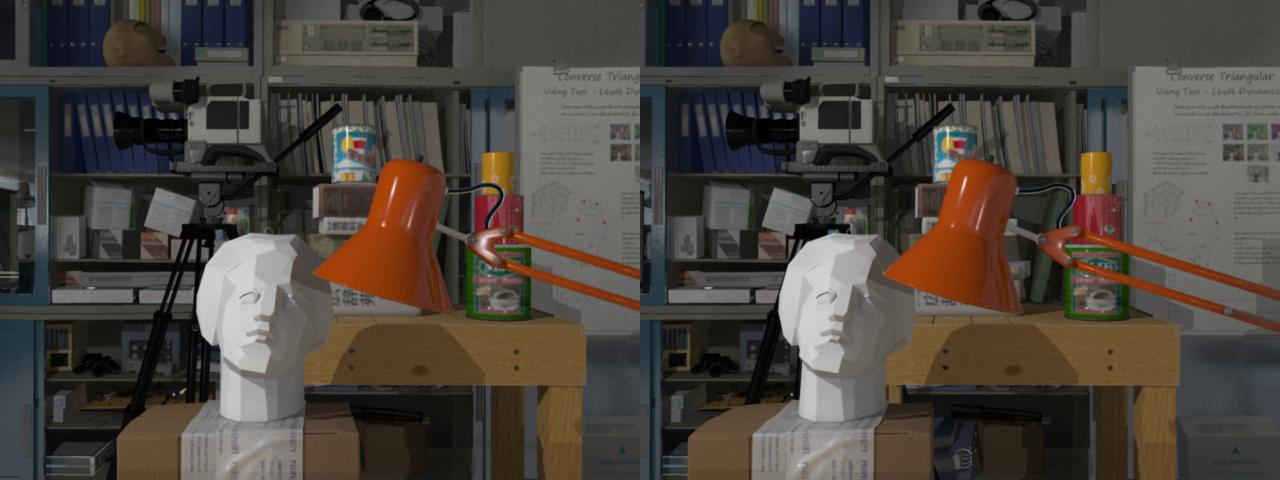
\includegraphics[width=1\textwidth]{./img/marked_03_DFT.png}
\caption{\small{stereo image marked with DFT algorithm with power equal to 0.3}}
\label{fig:dft03}
\end{figure}
\begin{figure}[h!]
\centering
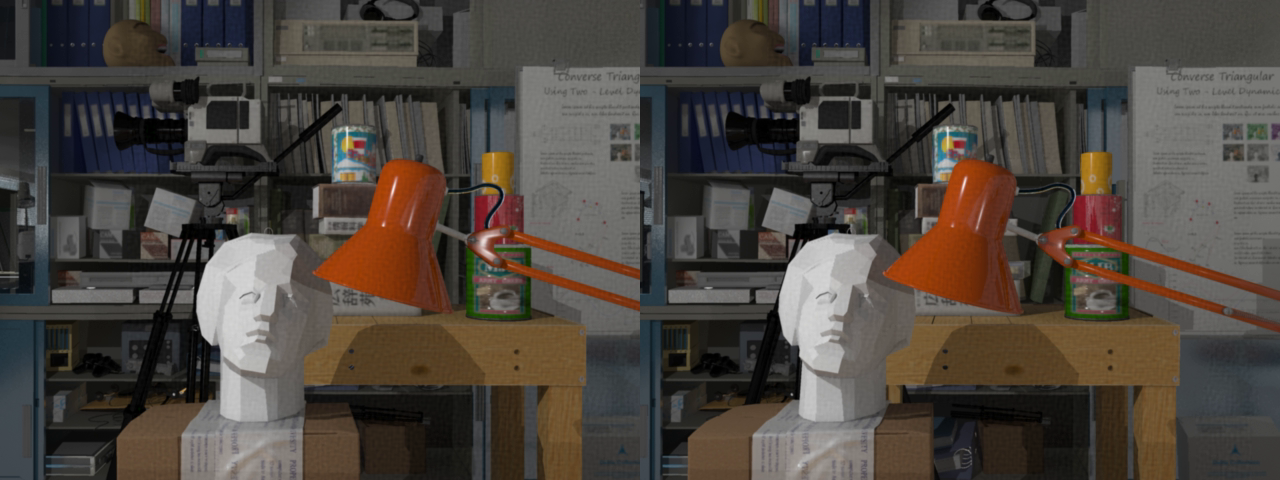
\includegraphics[width=1\textwidth]{./img/marked_05_DFT.png}
\caption{\small{stereo image marked with DFT algorithm with power equal to 0.5}}
\label{fig:dft05}
\end{figure}
\begin{figure}[h!]
\centering
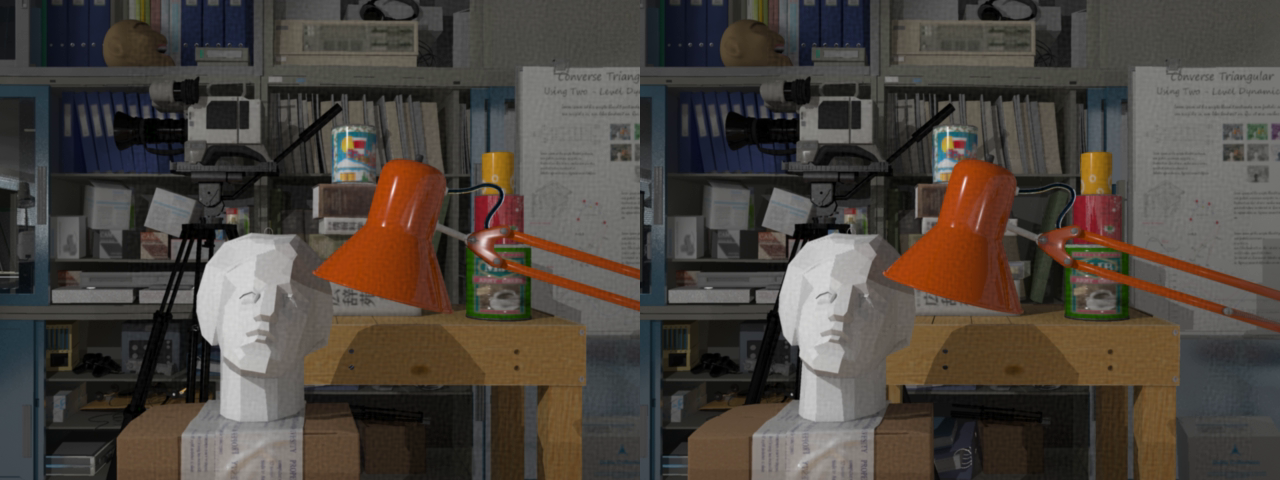
\includegraphics[width=1\textwidth]{./img/marked_06_DFT.png}
\caption{\small{stereo image marked with DFT algorithm with power equal to 0.6}}
\label{fig:dft06}
\end{figure}
\begin{figure}[h!]
\centering
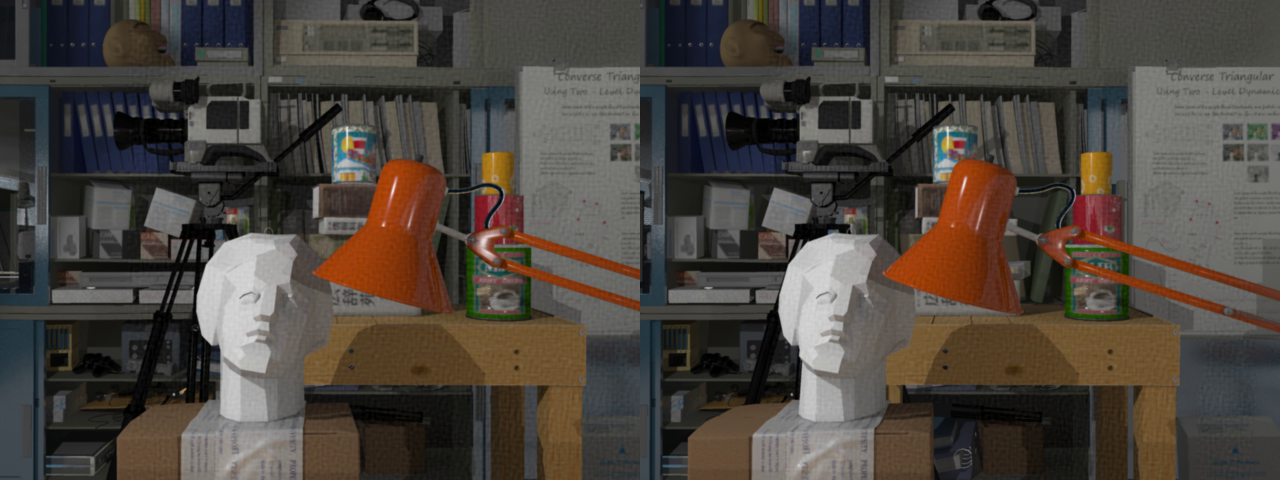
\includegraphics[width=1\textwidth]{./img/marked_07_DFT.png}
\caption{\small{stereo image marked with DFT algorithm with power equal to 0.7}}
\label{fig:dft07}
\end{figure}
\section{Stereo detection algorithm}

The detection of the watermark is performed with the detector implemented by Piva et al.\newline

As for the embedding process, to the left view the algorithm is applied without changes, yet, for the right view detection some adaptations are needed.\newline

First the detection algorithm computes the right-to-left disparity, then the right view is warped accordingly to ricreate the phase of the inserted watermark; to mantain the right phase the occluded zones are filled with the pixels of the recieved left view (taking under consideration that this little amount of image's pixel would not influence the detection).\newline
The created image is then processed by the threshold-based detection algorithm. 



